\documentclass[t, 11pt]{beamer}
\pdfmapfile{+sansmathaccent.map}
%%% Работа с русским языком
\usepackage{cmap}				
\usepackage{mathtext} 				
\usepackage[T2A]{fontenc}		
\usepackage[utf8]{inputenc}			
\usepackage[english,russian]{babel}	

\usetheme{Ilmenau}
\usecolortheme{lily} % Цветовая схема



%%% Работа с картинками
\usepackage{graphicx}

\usepackage{csquotes}

\hypersetup{				
	colorlinks=true,       	
	linkcolor=blue,          
	citecolor=black,       
	filecolor=magenta,      
	urlcolor=red           
}


\title{REGEX + scrapinng}
%\subtitle{...and it's applications}
%\author{Чувакин Сергей}
\date{24.9}
%\institute[<<Анализ больших данных в бизнесе, экономике и обществе>>]{<<Высшая школа экономики>>}
\institute{<<Высшая школа экономики>>}
\begin{document}
	\frame[plain]{\titlepage}
	\section{Outline}
	
	\begin{frame}
		\frametitle{\insertsection} 
		\begin{block} {}
			 
			\hyperlink{l1}{\beamerbutton{re templates}}
		\end{block}
			\begin{block}{}
		\hyperlink{l2}{\beamerbutton{scraping basics}}
		\end{block}
	\end{frame}
	
	\subsection{regex}
	\begin{frame} \label {l1}
		\frametitle{\insertsection} 
		\frametitle{\insertsubsection} 
		Регулярные выражения - язык описания шаблонов (patterns) для извлечения информации из текста.  
		\vspace{1cm}
		
		\emph{Pure} rule-based approach.
	\end{frame}

	
	\begin{frame}
		\frametitle{\insertsection}
		\frametitle{\insertsubsection}  
	\begin{itemize}

	\item Поиск точного совпадения.  

	\item Поиск шаблонного совпадения. 

	\item Возможность введения переменных.

	\item Жадность.

	\item Метасимволы.
	 \end{itemize}
	\end{frame}


	\begin{frame}
	\frametitle{\insertsection}
	\frametitle{\insertsubsection}  
Точное совпадение: 

\vspace{0.5cm}

Строка на вход  <<aaa bbb ccc>>

\vspace{0.5cm}

шаблон: r"a"

\vspace{0.5cm}

на выходе: [a, a, a]

\end{frame}


	\begin{frame}
	\frametitle{\insertsection}
	\frametitle{\insertsubsection}  
	[] - символ <<или>>
	
	\vspace{0.5cm}
	
	Строка на вход  <<aaa bbb ccc>>
	
	\vspace{0.5cm}
	
	шаблон: r"[ab]"
	
	\vspace{0.5cm}
	
	на выходе: [a, a, a, b, b, b]
	
\end{frame}


	\begin{frame}
	\frametitle{\insertsection}
	\frametitle{\insertsubsection}  
	() - группировка 
	
	\vspace{0.5cm}
	
	Строка на вход  <<aaa bbb ccc>>
	
	\vspace{0.5cm}
	
	шаблон: r"(aaa) bbb"
	
	\vspace{0.5cm}
	
	на выходе: [aaa]
	
\end{frame}

	\begin{frame}
	\frametitle{\insertsection}
	\frametitle{\insertsubsection}  
	Если группа не нужна, то в группе ставим :?
	
	\vspace{0.5cm}
	
	Строка на вход  <<aaa bbb ccc>>
	
	\vspace{0.5cm}
	
	шаблон: r"(aaa) (?:bbb)"
	
	\vspace{0.5cm}
	
	на выходе: [aaa]
	
\end{frame}

	\begin{frame}
	\frametitle{\insertsection}
	\frametitle{\insertsubsection}  
	Метасимволы
	\begin{itemize}
		\item $\backslash$d - все цифры [0-9]
		\item $\backslash$w - все буквы [a-Zа-Я]
		\item $\backslash$s - пробельные символы 
		\item  $\backslash$b - слова
	\end{itemize}
\end{frame}

	\begin{frame}
	\frametitle{\insertsection}
	\frametitle{\insertsubsection}  
	Метасимволы
	\begin{itemize}
		\item $\backslash$D - Не цифры [\^0-9]
		\item $\backslash$W - Не буквы [\^a-Zа-Я]
		\item $\backslash$S - Не пробельные символы 
		\item  $\backslash$B - Не слова
	\end{itemize}
\end{frame}
	\begin{frame}
	\frametitle{\insertsection}
	\frametitle{\insertsubsection}  
	Квантификаторы 
	\begin{itemize}
		\item \{n\} - n повторений
		\item \{n,m\} - минимум n, максимум m повторений
		\item \{n,\} - минимум n повторений
		\item \{,m\} - максимум m повторений
	\end{itemize}
\end{frame}

	\begin{frame}
	\frametitle{\insertsection}
	\frametitle{\insertsubsection}  
	Пример кватификатора
	
	\vspace{0.5cm}
	
	Строка на вход  <<На дворе - трава, на траве - дрова.>>
	
	\vspace{0.5cm}
	
	шаблон: r"[а-я]\{3,\}"
	
	\vspace{0.5cm}
	
	на выходе: ['дворе', 'трава', 'траве', 'дрова']
	
\end{frame}


	\begin{frame}
	\frametitle{\insertsection}
	\frametitle{\insertsubsection}  
	Синонимы кватификаторов 
	\begin{center}
		\begin{table}[]
			\begin{tabular}{c|c|c}
				\hline
				Синоним &Расшифровка &Квантификатор \\
				\hline
		+ & 1 и более раз &\{1,\}   \\
		* & 0 и более раз &\{0,\}   \\

		? &  0 или 1 раз& \{0,1\}  \\
  
			\end{tabular}
		\end{table}
	\end{center}
\end{frame}
	\begin{frame}
	\frametitle{\insertsection}
	\frametitle{\insertsubsection}  
	Жадность - по умолчанию регулярные выражения захватывают максимум символов, которые помещаются под шаблон.
	
	\vspace{0.5cm}
	
	Строка на вход  <<( dfghvb ) sdvsd ( sdcvkjnh ) sdvsd ( dkjhvgr ) sdvfv.>>
	
	\vspace{0.5cm}
	
	шаблон: r"$\backslash$(.+$\backslash$)"
	
	\vspace{0.5cm}
	
	на выходе: ['dfghvb ) sdvsd ( sdcvkjnh ) sdvsd ( dkjhvgr']
	
\end{frame}
\begin{frame}
	\frametitle{\insertsection}
	\frametitle{\insertsubsection}  
	Чтобы убрать жаность необходимо добавить ?
	
	\vspace{0.5cm}
	
	Строка на вход  <<( dfghvb ) sdvsd ( sdcvkjnh ) sdvsd ( dkjhvgr ) sdvfv.>>
	
	\vspace{0.5cm}
	
	шаблон: r"$\backslash$(.+?$\backslash$)"
	
	\vspace{0.5cm}
	
	на выходе: ['dfghvb', 'sdcvkjnh', 'dkjhvgr']
	
\end{frame}

\begin{frame}
	\frametitle{\insertsection}
	\frametitle{\insertsubsection}  
По умолчанию перенос строки ($\backslash$n) явялется концом поиска регулярного выражения.	

	\vspace{1cm}
(?s) в начале строки шаблона включает перенос строк.

\end{frame}

\subsection{scraping}
\begin{frame}
	\frametitle{\insertsection}
	\frametitle{\insertsubsection}  
	Скрапинг - процесс сбора информации с веб страниц.
	
	\vspace{1cm}
	
	Парсинг - процесс обработки текста, часто подразумевается разбор текста на составные части.  	
	
	
\end{frame}

\begin{frame}
	\frametitle{\insertsection}
	\frametitle{\insertsubsection}  
\begin{itemize}
	\item requests + bs4 - низкоуровневый поиск.
	\item selenium - имитация клиента.
	\item scrapy - готовое решение для скрапинга, основано на ассинхронных запросах.
	\end{itemize}  	
\end{frame}

\begin{frame}
	\frametitle{\insertsection}
	\frametitle{\insertsubsection}  
	Из чего состоит веб страница
	\begin{itemize}
		\item html 
		\item css
		\item js
	\end{itemize}  	
\end{frame}
\begin{frame}
	\frametitle{\insertsection}
	\frametitle{\insertsubsection}  
   Возможные проблемы:
	\begin{itemize}
		\item Скорость... 
		\item Тайминги, фризы.
		\item AJAX страницы.
	\end{itemize}  	
\end{frame}

	\begin{frame}
	\frametitle{\insertsection}
	\frametitle{\insertsubsection}
	
	
	%\vspace{1cm}
	\includegraphics[width=0.9\linewidth]{page.png}
	%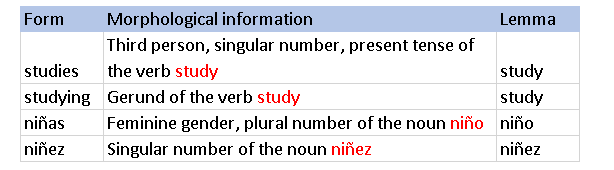
\includegraphics[width=0.7\linewidth]{lem.png}
\end{frame}

	\begin{frame}
	\frametitle{\insertsection}
	\frametitle{\insertsubsection}
	
	
	%\vspace{1cm}
	\includegraphics[width=0.9\linewidth]{page2.png}
	%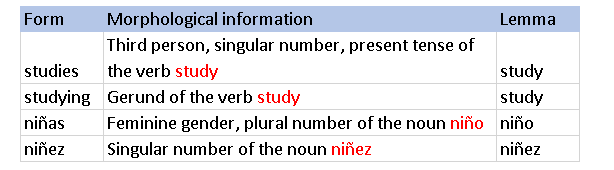
\includegraphics[width=0.7\linewidth]{lem.png}
\end{frame}
\end{document}